\documentclass[a4paper,12pt]{scrartcl}
\usepackage[utf8x]{inputenc}
\usepackage[T1]{fontenc} % avec T1 comme option  d'encodage c'est ben mieux, surtout pour taper du français.
%\usepackage{lmodern,textcomp} % fortement conseillé pour les pdf. On peut mettre autre chose : kpfonts, fourier,...
\usepackage[french]{babel} %Sans ça les guillemets, amarchpo
\usepackage{amsmath}
\usepackage{multicol}
\usepackage{amssymb}
\usepackage{tkz-tab}
\usepackage{exercice_sheet}



%\trait
%\section*{}
%\exo{}
%\question{}
%\subquestion{}

\date{}


% Title Page
\title{Devoir en classe, préformation Bac Pro}

\author{\rotatebox{10}{\textsc{Mathématiques}} \\ 40 minutes}

\begin{document}

\maketitle

{\Large Nom:} 
\hspace{60mm}
{\Large Prénom:}
\vspace{6mm}

Note : la calculatrice est autorisée. Donc sauf mention contraire, tout résultat donné sans la moindre étape de calcul ne sera pas pris en compte...

\section*{Algèbre}

\exo{Classer ces nombres dans l'ordre croissant:}

6 17 66 78 68 26 52 30

\lignes{1}

\exo{Effectuer les calculs suivants:}

\question{}
$5+3+2-4+8$
\lignes{1}


\question{}
$(4+7) \times 3 + 4 \times 2$
\lignes{1}

\question{}
$(4+1)(2+7)$
\lignes{1}

\question{Donner la valeur exacte, en une seule fraction:}
$\dfrac{7}{12} + \dfrac{11}{8}$
\lignes{1}

\exo{Développer et réduire les écritures suivantes:}

\question{}$(x+1)(x-2)$
\lignes{1}

\question{}
$(1-x)(2x+1)$
\lignes{1}

\exo{Simplifier (la réponse doit être sous forme de puissance):}

\question{}
$10^{7} \times 10^{12}$
\lignes{1}

\question{}
$\dfrac{4^{13}}{4^{2}}$
\lignes{1}

\exo{Donner l'écriture scientifique des nombres suivants (aucun détail de calcul n'est demandé):}

\question{}
$4534$
\lignes{1}

\question{}
$0.000543$
\lignes{1}

\question{}
$18 \times 10^{5}$
\lignes{1}

\section*{Géométrie}

\exo{Rectangles}
On considère un rectangle de 8cm de large et 12cm de long.

\question{Donner le périmètre $\mathcal{P}_1$ et l'aire $\mathcal{A}_1$ de ce rectangle}
\lignes{1}

\question{Ce rectangle subit un agrandissement de facteur $k = 1.5$. Donner le périmètre $\mathcal{P}_2$ et l'aire $\mathcal{A}_2$ de ce nouveau rectangle} 
\lignes{2}

\exo{Triangles}

\begin{center}
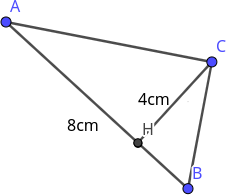
\includegraphics[width=0.3\linewidth]{pics/triangle.png}
\end{center}

Le triangle $ABC$ a pour base $[AB]$, de longueur 8cm et pour hauteur $[HC]$, de longueur 4cm. 

Quelle est son aire? Détailler les calculs.
\lignes{2}

\question{Quelle est la définition d'une hauteur dans un triangle?}
\lignes{2}

\question{Quelle est la définition d'une médiane dans un triangle?}
\lignes{2}

\exo{Quadrilatères}

Pour cet exercice, vous pourrez répondre soit par écrit soit en dessinant les codages sur les figures.

\question{Rappeler les propriétés d'un parallélogramme. }
\lignes{1}

\begin{center}
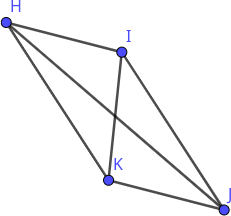
\includegraphics[width=0.3\linewidth]{pics/parallelogramme.png}
\end{center}

\question{Un losange est un parallélogramme particulier. Il hérite donc de ses propriétés, mais il en a en plus. Quelles son-elles?}
\lignes{1}

\begin{center}
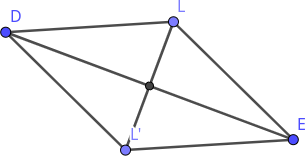
\includegraphics[width=0.4\linewidth]{pics/losange.png}
\end{center}

\trait

\begin{center}
Fin.
\end{center}

\end{document}

